\begin{Ueberlieferung}%
{\textit{L}}Aufzeichnung: LH XXXVII 4 Bl. 51-52.
1 Bog. 2\textsuperscript{o}.
2 S. Textfolge: Bl. 52~v\textsuperscript{o}, 51~r\textsuperscript{o}.
Bl. 51~v\textsuperscript{o} und 52~r\textsuperscript{o} sind leer.
Bl. 52~v\textsuperscript{o} überliefert zudem das Stück \textit{LSB} VII, 1 N. 46.\cite{01085}
Ein Wasserzeichen auf Bl. 52.
Dort auch oberer Rand beschnitten (mit Textverlust in \textit{LSB} VII, 1 N. 46\cite{01085}).\\%
Cc 2, Nr. 967 A
\end{Ueberlieferung}
\vspace*{8mm}
\begin{Datierungsgruende}%
Das vorliegende Stück N. 26 % F/8 = 037,04_051-052
ist mit Fragen der Bruch- und Zugfestigkeit un\-ela\-sti\-scher Körper befasst.
Damit weist N. 26 % F/8 = 037,04_051-052
eine unmittelbare Verbindung mit den Themen auf,
die in den Stücken N. 19-25, % F/1-7 = 037,05_201, 037,05_204, 037,05_202-203, 037,05_209, 037,05_210, 037,05_211, 037,05_207-208
zumeist in Anlehnung an Überlegungen aus Galielis\protect\index{Namensregister}{\textso{Galilei} (Galilaeus, Galileus), Galileo 1564-1642}
\textit{Discorsi e dimostrazioni matematiche},
behandelt werden.
Ferner liegt im Textträger von N. 26 % /F8 = 037,04_051-052
das gleiche Wasserzeichen vor wie auf den Bogen,
welche die Stücke N. 19-21 % F/1-3 = 037,05_201, 037,05_204, 037,05_202-203
und N. 23-25 % F/5-7 = 037,05_210, 037,05_211, 037,05_207-208
überliefern. Demgemäß ist die für N.~19-25 % F/1-7 = 037,05_201, 037,05_204, 037,05_202-203, 037,05_209, 037,05_210, 037,05_211, 037,05_207-208
vorgeschlagene Datierung grundsätzlich auch für N. 26 % F/8 = 037,04_051-052
zu übernehmen.
\newline%
\hspace*{7,5mm}%
Dies zieht eine Umdatierung des auf Bl. 52~v\textsuperscript{o} überlieferten Stücks \textit{LSB} VII, 1 N.~46\cite{01085} nach sich.
In diesem letzteren Stück, für welches ursprünglich Juni-August 1674 als Entsteh\-ungszeit angenommen wurde,
geht es um das von Jacques Ozanam\protect\index{Namensregister}{\textso{Ozanam} (Osanna), Jacques 1640-1717}
\glqq neulich\grqq~(\textit{nuper}) gelöste Problem,
drei vierte Potenzen in arithmetischer Folge zu finden.
Leibniz' Brief an Heinrich Oldenburg\protect\index{Namensregister}{\textso{Oldenburg} (Grubendol), Heinrich 1618-1677} vom 8. März 1673
berichtet von derartigen zahlentheoretischen Problemen,
insbesondere vom sogenannten Sechsquadrate-Problem (\textit{LSB} III, 1 N. 9, S. 42.8-26\cite{00251}).
Erst in den Monaten Juni-August 1674 wendet sich Leibniz selbst diesem Problem näher zu.
Dem entspricht, dass er in \textit{LSB} VII, 1 N. 45\cite{01086} erneut das Problem von N. 46\cite{01085}
mit der Bemerkung formuliert: \glqq Dieses Problem hat Ozanam gelöst.\grqq~In der Tat lag die Lösung nunmehr über ein Jahr zurück.
\newline%
\hspace*{7,5mm}%
Aus der gemeinsamen Überlieferung mit \textit{LSB} VII, 1 N. 46\cite{01085} lässt sich jedoch schließen,
dass auch das vorliegende Stück N. 26 % F/8 = 037,04_051-052
nicht viel früher als Anfang März 1673 entstanden sein dürfte.
% Die in \textit{LSB} VII, 1 N. 46\cite{01085} edierten Zeilen von Bl. 52~v\textsuperscript{o} sind auf Juni-August 1674 datiert.
% Das vorliegende Stück dürfte in zeitlicher Nähe entstanden sein.
\end{Datierungsgruende}
%%
%%
% \newpage% PR: Rein provisorisch !!!
\count\Afootins=1200
\count\Bfootins=1200
\count\Cfootins=1200
\pstartfirst
% \pstart% PR: Rein provisorisch !!!
\noindent%
[52~v\textsuperscript{o}] Sit Tabula lignea lata ut 2. alta \edtext{magis}{\lemma{}\Bfootnote{magis \textit{erg.} \textit{L}}} ut 6.
infixa muro\protect\index{Sachverzeichnis}{murus}
\edtext{primum ut altitudo}{\lemma{primum ut}\Bfootnote{\textit{(1)}\ latitudo \textit{(2)}\ altitudo \textit{L}}}
ut 6 sit parallela,
latitudo autem ut 2. perpendicularis
horizonti ut in fig. 2.
\edtext{Ponatur prisma in fig. 2. altitudinis}{\lemma{Ponatur}\Bfootnote{%
\textit{(1)}\ altitudo \textit{(2)}\ prisma in fig. 2. altitudinis \textit{L}}} $\displaystyle ab$ ut 2. latitudinis etiam ut 2.
nempe $\displaystyle bc.$ seu rectangulum solidum $\displaystyle abcd$
basin habens quadratam $\displaystyle abc.$ rumpi
\edtext{posse libra\protect\index{Sachverzeichnis}{libra}}{\lemma{posse}\Bfootnote{\textit{(1)}\ vi ut \textit{(2)}\ libra\protect\index{Sachverzeichnis}{libra} \textit{L}}} 
1. Ergo tota Tabula $\displaystyle adef$ rumpetur
libris~3\protect\index{Sachverzeichnis}{libra}.
\pend
\newpage% PR: Rein provisorisch !!!
%\vspace*{1em}% PR: Rein provisorisch !!!
\pstart
% \begin{minipage}[t]{0.2\textwidth}
% \hspace*{5mm}
\noindent%
\centering%
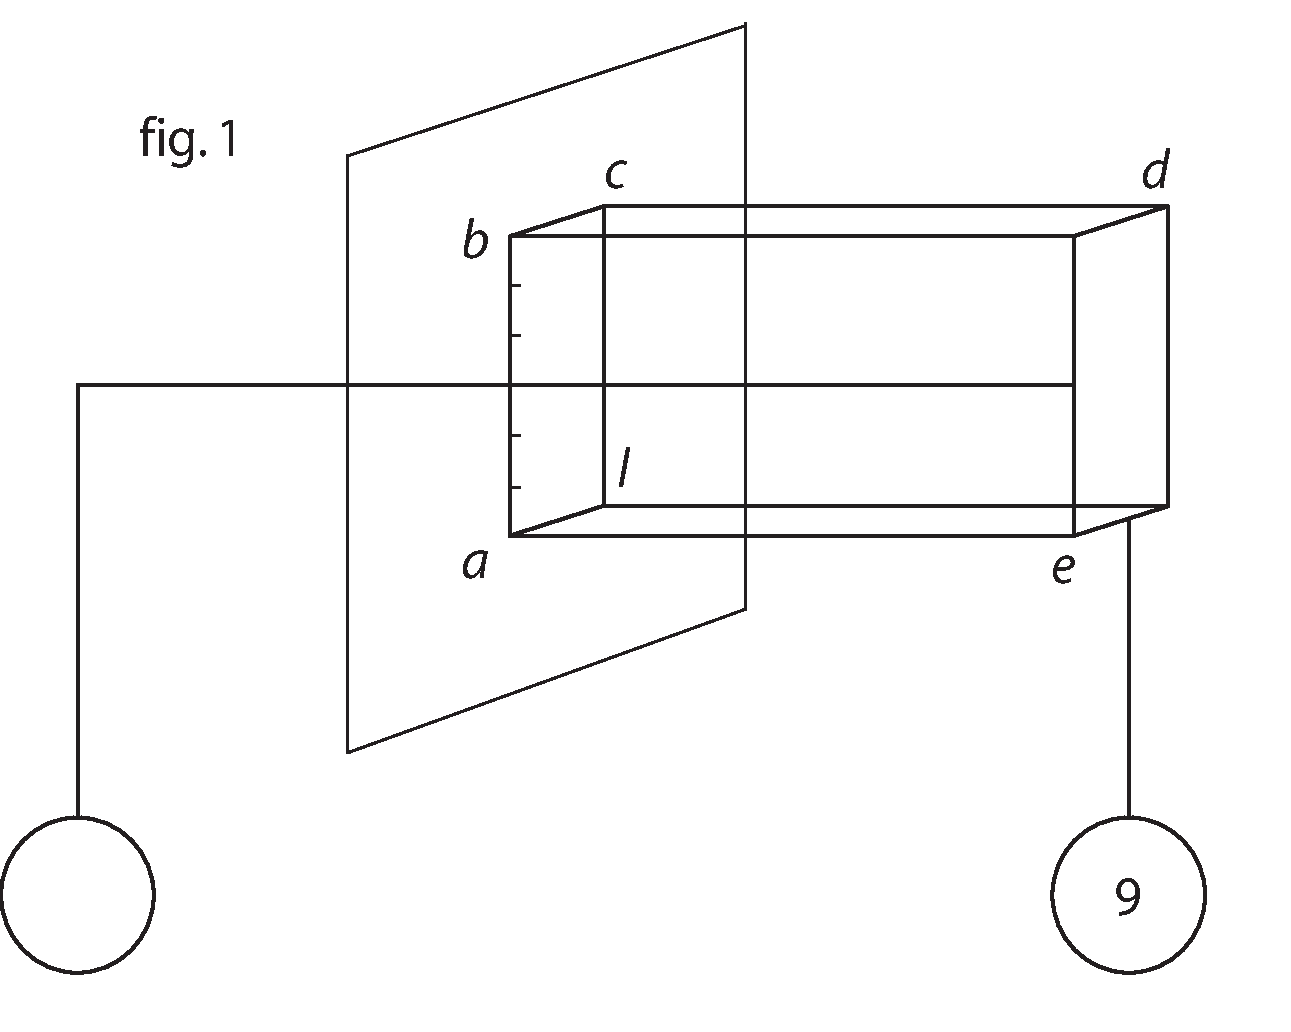
\includegraphics[width=0.64\textwidth]{images/LH037,04_051-052d-1.pdf}
% \newline
%\hspace*{3mm}
% \rule[0pt]{0mm}{0mm}%
% [\textit{Fig. 1}]
% \end{minipage}
% \hspace*{40mm}
\pend
% \newpage% PR: Rein provisorisch !!!
\vspace*{2.5em}% PR: Rein provisorisch !!!
\pstart
% \begin{minipage}[t]{0.2\textwidth}
% \hspace*{5mm}
\noindent%
\centering%
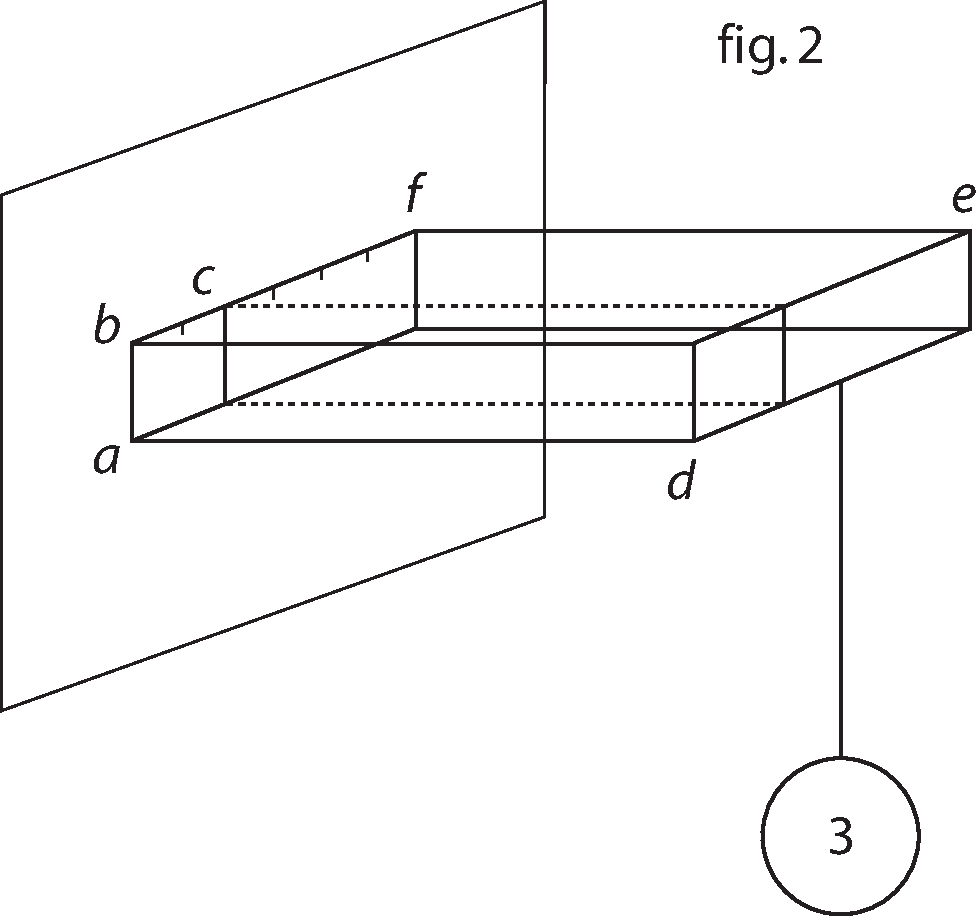
\includegraphics[width=0.49\textwidth]{images/LH037,04_051-052d-2.pdf}
% \newline
% \hspace*{3mm}
% \rule[0pt]{0mm}{0mm}% PR: Rein provisorisch !!!
% [\textit{Fig. 2}]
% \end{minipage}
\pend
\vspace*{2.5em}% PR: Rein provisorisch !!!
%\newpage
\pstart
At \setline{1}in fig. 1 ubi Tabula erecta statuta est, seu latitudo ejus
horizonti parallela, ibi latitudo eadem quae in fig. 2 prismatis $\displaystyle abcd$
quod statueramus pondere rumpi librae\protect\index{Sachverzeichnis}{libra} 1. altitudo vero est tripla. Ergo
pondere opus est librarum\protect\index{Sachverzeichnis}{libra} novem.
\pend
\newpage
\pstart%
%\rule[0mm]{0mm}{4mm}% PR: Rein provisorisch !!!
Et generaliter demonstrari potest rationem
esse quae est altitudinis ad latitudinem, esto
\edtext{enim latitudo $\displaystyle a,$}{\lemma{enim}\Bfootnote{ \textit{(1)}\ altitudo 1. \textit{(2)}\ latitudo \textit{(a)}\ minor \textit{(b)}\ $\displaystyle a$ \textit{L}}}
\edtext{altitudo $\displaystyle b.$ $\displaystyle a^{2}$}{\lemma{altitudo $\displaystyle b.$}\Bfootnote{\textit{(1)}\ Prisma \textit{(2)}\ Quadr. \textit{(3)}\ $a^{2}$ ut firmitatis ut 1. \textit{(4)}\ $a^{2}$ \textit{L}}}
firmitatis\protect\index{Sachverzeichnis}{firmitas} ut 1 lib.
%\rule[0mm]{0mm}{6mm}% PR: Rein provisorisch !!!
\edtext{Ergo}{\lemma{Ergo}\Bfootnote{\textit{erg. L}}}
\edtext{$\displaystyle ab$
\edtext{jacentis}{%
\lemma{jacentis}\Cfootnote{Gemeint ist offenbar ein Prisma.}}}{%
\lemma{$\displaystyle ab$}\Bfootnote{\textit{(1)}\ horizontale \textit{(2)}\ jacentis \textit{L}}}
firmitatis\protect\index{Sachverzeichnis}{firmitas} ut \protect\rule[-4mm]{0mm}{10mm}$\displaystyle\frac{b}{a}$ lib.
% \pend
% \pstart%
Et \textit{ab} erecti $\displaystyle\frac{bb}{aa}$ lib.
\protect\rule[-4mm]{0mm}{10mm}Jam $\displaystyle\frac{b^{2}}{a^{2}}$ ad $\displaystyle\frac{b}{a}.$
seu $\displaystyle\frac{b^{2}}{a}$ ad $\displaystyle\frac{b}{1}.$
seu $\displaystyle\frac{b}{a}$ ad 1.
seu ut $b$ \edtext{ad $\displaystyle a$.\\%
\indent%
Rectangulo solido}{\lemma{ad $\displaystyle a$}\Bfootnote{\textit{(1)}\ Prismate  \textit{(2)}\ Rectangulo  \textit{L}}}
basin quadratam habente sumto,
esto ejus altitudo $\displaystyle a$, latitudo $\displaystyle a$, resistentia\protect\index{Sachverzeichnis}{resistentia} 1
\edtext{\Pfund. quadrati  $\displaystyle a^{2}.$ Esto}{\lemma{\Pfund.}\Bfootnote{\textit{(1)}\  Esto basis \textit{(2)}\  quadratum \textit{(3)}\ duplicetur altitudo, \textit{(4)}\ quadrati  $\displaystyle a^{2}.$ Esto \textit{L}}}
latus quadrati $\displaystyle 2a$. Erit ejus quadratum $\displaystyle 4a^{2}$. Sed ponatur
duplicata tantum esse altitudo, retenta latitudine, erit basis $\displaystyle 2a^{2}$. Cumque
$\displaystyle a^{2}$ sit firmitatis\protect\index{Sachverzeichnis}{firmitas} ut \edtext{[2.]}{\lemma{}\Bfootnote{1.\textit{\ L \"{a}ndert Hrsg.}}} erit $\displaystyle 2a^{2}$ firmitatis\protect\index{Sachverzeichnis}{firmitas} ut 4. et $\displaystyle 4a^{2}$ firmitatis\protect\index{Sachverzeichnis}{firmitas} ut
8. Sunt ergo in ratione triplicata. \edtext{$\displaystyle b$ autem distet a centro staterae\protect\index{Sachverzeichnis}{statera} $\displaystyle a$ quantum in fig. 1. $\displaystyle d$ ab $\displaystyle a.$}{\lemma{}\Bfootnote{$\displaystyle b$ autem [...]  ab $\displaystyle a.$\textit{ erg. L}}}
\pend
\vspace{2em}% PR: Rein provisorisch !!!
\pstart
% \begin{minipage}[t]{0.2\textwidth}
\centering
\noindent
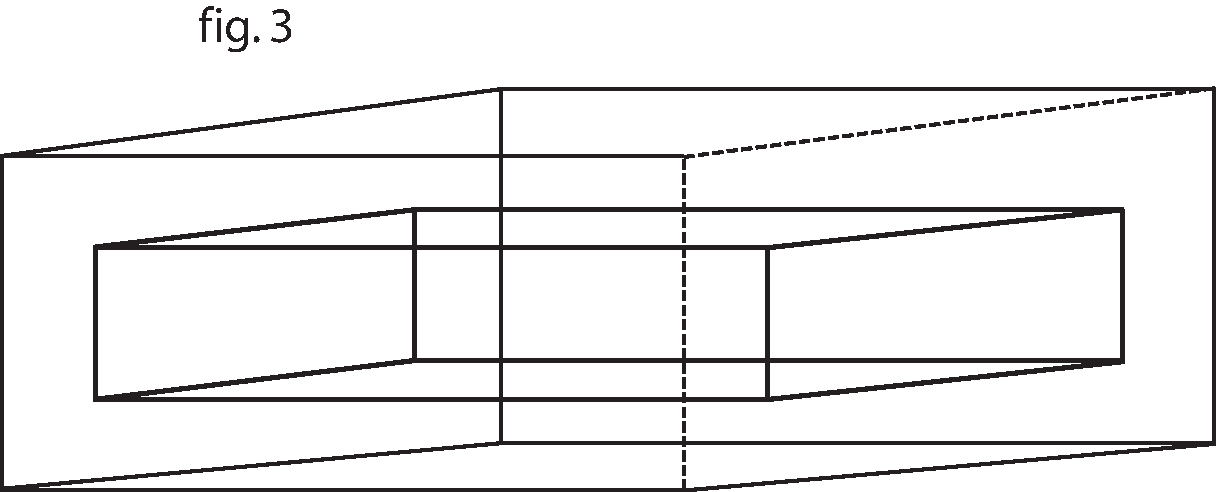
\includegraphics[width=0.68\textwidth]{images/LH037,04_051-052d-3.pdf}
% \vspace*{1.5em}% PR: Rein provisorisch !!!
% \newline%
% [\textit{Fig. 3}]
% \end{minipage}
\pend
\vspace{2.0em}
%\newpage% PR: Rein provisorisch !!!
\pstart% 
Quaeritur \setline{9}quae sit ratio rupturae centralis\protect\index{Sachverzeichnis}{ruptura centralis} ad
\edtext{liberam}{\lemma{liberam}\Cfootnote{Die Wortform \textit{libera} für \textit{libra} ist nicht klassisch.
Laut \cite{01089}C. \textsc{Du Cange}, \textit{Glossarium mediae et infimae latinitatis}, Niort 1883-1887, Bd. V, Sp. 90b (\textit{sub voce})
ist sie aber für das Mittellatein belegt.}}
ut si Trabs\protect\index{Sachverzeichnis}{trabs}
in fig. 1 ita appendatur in fig. 4 vel saltem homo eam recta e muro\protect\index{Sachverzeichnis}{murus} educere conetur.
\edtext{Et primum data centrali resistentia\protect\index{Sachverzeichnis}{resistentia} invenire liberam:}{\lemma{Et primum [...] liberam:}\Bfootnote{ \textit{ erg. L}}}
Reducatur basis $\displaystyle abc$
\edtext{fig. 1}{\lemma{}\Bfootnote{fig. 1 \textit{erg.} \textit{L}}}
quaecunque sit,
\edtext{in rectangulum}{\lemma{in}\Bfootnote{\textit{(1)}\ prisma \textit{(2)}\ rectangulum \textit{L}}}
per methodum\protect\index{Sachverzeichnis}{methodus}
\edtext{superiorem determineturque}{\lemma{superiorem}\Bfootnote{ \textit{(1)}\ . Fiat Tabula lon  \textit{(2)}\ . Sumatur in fig. 6 \textit{(3)}\ determineturque \textit{L}}} pondus aequilibrans ejus firmitati\protect\index{Sachverzeichnis}{firmitas}
ut est 9 in fig. 1.
\edtext{%
Fiat in fig. 5 statera\protect\index{Sachverzeichnis}{statera} ex qua
suspendatur dictum \edtext{pondus 9 in $\displaystyle b.$ et alterum staterae brachium\protect\index{Sachverzeichnis}{brachium} sit Tabula lignea}%
{\lemma{pondus 9}\Bfootnote{%
\textit{(1)}\ ex altero staterae brachio eadem sit a centro $\displaystyle a$ distantia quae est $\displaystyle b.$ nempe ex $\displaystyle c.$ Suspendatur %
\textit{(2)}\ in $\displaystyle b.$ [...] lignea \textit{L}}}
\edtext{horizontalis}{\lemma{horizontalis}\Bfootnote{\textit{erg. L}}}
tantae longitudinis $\displaystyle cd$
\edtext{(fig. 5)}{\lemma{(fig. 5)}\Bfootnote{\textit{erg. L}}}
quanta est \edtext{$\displaystyle ad$\edtext{ (fig. 1)}{\lemma{$\displaystyle ad$ (fig. 1)}\Bfootnote{\textit{erg. L}}}%
}{\lemma{$\displaystyle ad$ (fig. 1)}\Cfootnote{In [\textit{Fig. 1}] hat Leibniz mit $\displaystyle d$ ursprünglich die rechte, vordere, untere Ecke des Balken\-endes bezeichnet, so dass $\displaystyle ad$ dort die Länge des Balkens war. Später hat er in [\textit{Fig. 1}] dieses $\displaystyle d$ gestrichen und mit dem gleichen Buchstaben die rechte, hintere, obere Ecke des Balkenendes bezeichnet.}}
distantia ex qua suspensum pondus 9 in fig. 1.
tantae latitudinis $\displaystyle ef$ (fig. 5)
quanta $\displaystyle bc$ seu latitudo basis rumpendae fig. 1.
tantae denique crassitiei\protect\index{Sachverzeichnis}{crassities}\edlabel{37,04_051-052_az-1}
\edtext{$\displaystyle ef$ (fig. 5)}%
{{\xxref{37,04_051-052_az-1}{37,04_051-052_az-2}}{\lemma{crassitiei}\Bfootnote{%
\textbar\ $\displaystyle ef$ (fig. 5) \textit{erg.} \textbar\ ut aequiponderet \textit{L}}}}%
}{\lemma{Fiat [...] (fig. 5)}\Cfootnote{Mit \glqq fig. 5\grqq~bezeichnet Leibniz in dieser Passage die gestrichene Variante von [\textit{Fig. 4b}].
Die Breite $\displaystyle ef$ in der ungültigen \glqq fig. 5\grqq~entspricht der Breite $\displaystyle ec$ in [\textit{Fig. 4b}].}}
ut aequiponderet\edlabel{37,04_051-052_az-2}
\edtext{ponderi 9. Quod}{\lemma{ponderi 9.}\Bfootnote{\textit{(1)}\ fiat alia jam Tabula ejus \textit{(2)}\ Quod \textit{L}}}
facile determinatur, si enim sumatur initio crassitiei\protect\index{Sachverzeichnis}{crassities} cujuscunque pro et pondere sui, ratio
ponderis dabit, quantum augenda sit crassities\protect\index{Sachverzeichnis}{crassities}, ut
% \edtext{
aequilibrent.
\pend
\vspace*{4.0em}% PR: Rein provisorisch !!!
\pstart
\begin{minipage}[t]{0.4\textwidth}
\noindent
\centering
\hspace{-10mm}
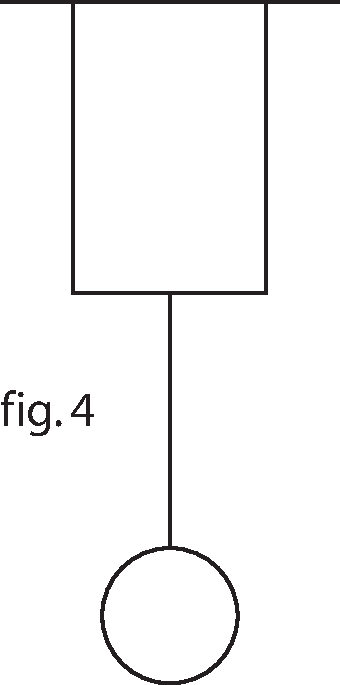
\includegraphics[width=0.42\textwidth]{images/LH037,04_051-052d-4.pdf}\\
\centering
\vspace*{0.5em}
\hspace{-10mm}
[\textit{Fig. 4a}]
\end{minipage}
\begin{minipage}[t]{0.6\textwidth}
\noindent
%\centering
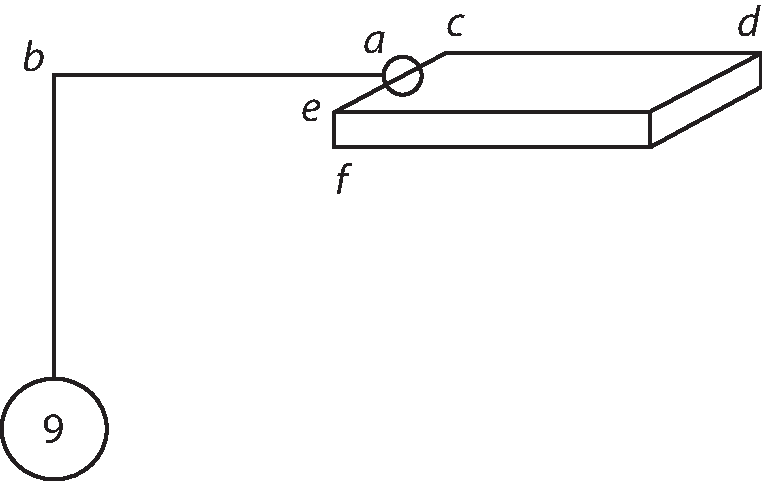
\includegraphics[width=0.85\textwidth]{images/LH037,04_051-052d-5.pdf}\\
\centering
\vspace*{0.5em}
\hspace{0mm}
[\textit{Fig. 4b}]
\end{minipage}
\edtext{}{\lemma{\hspace*{1,8mm}[\textit{Fig. 4b}]}\killnumber\Cfootnote{Eine gestrichene Variante dieser Abbildung trägt in der Handschrift die Bezeichnung \glqq fig. 5\grqq~.}}
\pend
\newpage
%\vspace*{4.0em}% PR: Rein provisorisch !!!
%\vspace*{0.5em}%
\pstart%
\noindent%
\lbrack \textit{Nachfolgend kleingedruckter Text gestrichen}:\rbrack
\pend
\count\Afootins=1000
\count\Bfootins=1000
\count\Cfootins=1000
%\vspace{0.5mm}%
\pstart%
\noindent%
\footnotesize%
Jam fiat alia
[51~r\textsuperscript{o}]
Tabula
\edtext{similis basi $\displaystyle abc$ fig. 1.}{\lemma{similis [...] fig. 1.}\Bfootnote{\textit{erg. L}}}
ejusdem crassitiei\protect\index{Sachverzeichnis}{crassities}
cujus \edtext{%
$\displaystyle cf$ (fig. 5)\edtext{}{\lemma{(fig. 5)}\Bfootnote{\textit{erg. L}}}
nempe crassitiei\protect\index{Sachverzeichnis}{crassities}
$\displaystyle ef$ (fig. 5)\edtext{}{\lemma{(fig. 5)}\Bfootnote{\textit{erg. L}}}%
}{\lemma{$\displaystyle cf$ (fig. 5) [...] $\displaystyle ef$ (fig. 5)}\Cfootnote{%
Mit den (nachträglich ergänzten) Bezeichnungen \glqq fig. 5\grqq~verweist Leibniz offenbar auf unterschiedliche Diagramme:
zunächst tatsächlich auf \textit{fig. 5}, dann aber auf die gestrichene Variante von [\textit{Fig. 4b}].}}
per pondus 9 inventae
per \edtext{calculatio[\textit{!}],\protect\index{Sachverzeichnis}{calculatio}
hoc loco tabulae $\displaystyle cd$ appendatur
\edtext{fig. 5}{\lemma{fig. 5}\Cfootnote{Der Bezug ist wieder tatsächlich \textit{fig. 5}.}}
staterae,\protect\index{Sachverzeichnis}{statera}}{\lemma{calculatio,}\Bfootnote{%
\textit{(1)}\ hoc loco ponderis 9 appendatur ex $\displaystyle b.$ Ea ejusdem quoque latitudinis,
\textit{(2)}\ hoc loco %
\textit{(a)}\ ponderis 9 %
\textit{(b)}\ tabulae [...] fig. 5 %
\textit{(aa)}\ ex $\displaystyle b$ brachio staterae %
\textit{(bb)}\ staterae \textit{L}}}
quo facto quae erit ratio ponderum inter duas Tabulas,
ea erit virium ad rupturam absolutam\protect\index{Sachverzeichnis}{ruptura absoluta} necessariarum ad vires necessarias ad centralem.
Determinata \edtext{jam de habita}{\lemma{jam}\Bfootnote{\textit{(1)}\ absoluta \textit{(2)}\ de habita \textit{L}}}
resistentia\protect\index{Sachverzeichnis}{resistentia} unius determinatur omnium,
sunt enim inter se
\edtext{ut sectiones rupturae.\protect\index{Sachverzeichnis}{ruptura}}{\lemma{ut}\Bfootnote{\textit{(1)}\ bases \textit{(2)}\ sectiones rupturae. \textit{L}}}
\pend
\pstart
\footnotesize%
Et haec ratiocinatio\protect\index{Sachverzeichnis}{ratiocinatio} est sine omni calculo centri 
gravitatis\protect\index{Sachverzeichnis}{centrum gravitatis}. Inverso modo ex 
\edtext{data}{\lemma{data}\Bfootnote{\textit{erg. L}}} Absoluta determinabis resistentiam
\edtext{respectivam.\protect\index{Sachverzeichnis}{resistentia respectiva}
Fundamentum\protect\index{Sachverzeichnis}{fundamentum}}{\lemma{respectivam.}\Bfootnote{\textit{(1)}\ In simplici cy  \textit{(2)}\ Si per viam centri gravitatis\protect\index{Sachverzeichnis}{centrum gravitatis} ra  \textit{(3)}\  Investigemus  \textit{(4)}\  Fundamentum\protect\index{Sachverzeichnis}{fundamentum} \textit{L}}} hoc est, cognita \edtext{ex potentia}{\lemma{ex}\Bfootnote{\textit{(1)}\ pondere \textit{(2)}\ potentia \textit{L}}} 9 resistentia\protect\index{Sachverzeichnis}{resistentia} ad rupturam centralem\protect\index{Sachverzeichnis}{ruptura centralis},
\edtext{fit loco}{\lemma{fit}\Bfootnote{\textit{(1)}\ aliud \textit{(2)}\ loco \textit{L}}} potentiae 9 prisma quod proprio pondere ad rupturam\protect\index{Sachverzeichnis}{ruptura} sufficeret, aequiponderans scilicet ipsi 9 sua gravitatione. Hoc prisma est virium 
\edtext{longitudine}{\lemma{longitudine}\Bfootnote{\textit{erg. L}}} eodem modo crescentium ut resistentiae\protect\index{Sachverzeichnis}{resistentia} sectionis rupturae\protect\index{Sachverzeichnis}{ruptura} crescunt. Cum ergo sunt ejusdem latitudinis sunt in longitudinum ratione. Hinc si corpora sunt cylindrica centra gravitatum\protect\index{Sachverzeichnis}{centrum gravitatis} sunt in medio. Et proinde pondus 9 \edtext{fig. 1}{\lemma{fig. 1}\Bfootnote{\textit{ erg. L}}} in medio \edtext{$e$}{\lemma{$e$}\Bfootnote{ \textit{ erg. L}}} suspensum aequabitur Trabi\protect\index{Sachverzeichnis}{trabs} \textit{ad} horizontaliter.
\pend
\vspace*{0.9em}% PR: Rein provisorisch !!!
% \newpage% PR: Rein provisorisch !!!
\pstart
% \begin{wrapfigure}{l}{0.3\textwidth}
\centering%
\noindent%
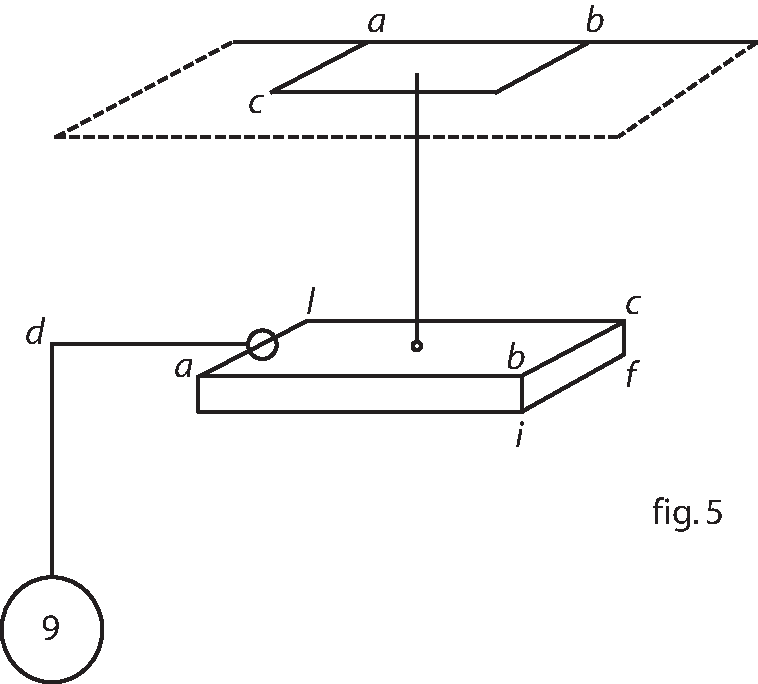
\includegraphics[width=0.49\textwidth]{images/LH037,04_051-052d-6.pdf}
% \newline%
% \rule[0pt]{0mm}{0mm}% PR: Rein provisorisch !!!
% [\textit{Fig. 5}]
% \end{wrapfigure}
\pend
\newpage
%\vspace*{2.5em}% PR: Rein provisorisch !!!
\pstart
\normalsize
Ut inquiratur ratio consistentiae centralis ad liberam,
ac per consequens, ut data centrali inveniri possit libera,
et contra, sic agendum est:
Data est nobis in \textso{fig. 1} consistentia
\edtext{centralis aequivalens ponderi ad eam rumpendam sufficienti 9.}{\lemma{centralis}\Bfootnote{\textit{(1)}\ ponderis 9.\ \textit{(2)}\ aequivalens [...] sufficienti 9.\ \textit{L}}}
Hoc pondus 9 in \textso{fig. 5} suspendatur ex staterae\protect\index{Sachverzeichnis}{statera} $\displaystyle dac.$ centri $\displaystyle a.$ brachii\protect\index{Sachverzeichnis}{brachium} $\displaystyle ad.$ \edtext{extremitate $\displaystyle d.$ ita}{\lemma{extremitate $\displaystyle d.$}\Bfootnote{\textit{(1)}\ ex alterius brachii $\displaystyle fi.$ extremitate $\displaystyle i.$ aequidistante ab $\displaystyle f.$ suspendatur Tabula $\displaystyle acb$ parallela horizonti, \textbar\ cujus facies \textit{erg.} \textbar\ similis \textbar\ et aequalis \textit{erg.} \textbar\ sectioni divulsionis\protect\index{Sachverzeichnis}{divulsio} $\displaystyle abc$ in fig. 1 similiterque posita, ita ut $\displaystyle al$ ibi est linea minime resistens, hic sit minime \textit{(2)}\ ita \textit{L}}}
ut $\displaystyle ad$ fig. 5 sit = $\displaystyle ad$ fig. 1. et facies $\displaystyle lcb$ Tabulae $\displaystyle alcfb$ sit aequalis et similis sectioni divulsionis\protect\index{Sachverzeichnis}{divulsio} $\displaystyle abcl.$ et ita posita ad centrum vel axem staterae\protect\index{Sachverzeichnis}{statera} in fig. 5. uti $\displaystyle abcl$ est posita ad centrum vel axem divulsionis\protect\index{Sachverzeichnis}{divulsio} in fig. 1. crassitiei\protect\index{Sachverzeichnis}{crassities} autem
\edtext{$\displaystyle cf$}{\lemma{$\displaystyle cf$}\Bfootnote{\textit{erg. L}}}
tantae, ut aequiponderet ponderi 9.
Quo facto Tabula
\edtext{$\displaystyle alcfb$ par erit superandae pondere suo resistentiae\protect\index{Sachverzeichnis}{resistentia}}{\lemma{$\displaystyle alcfb$}\Bfootnote{\textit{(1)}\ capax erit ad superandam pondere proprio resistentiam \textit{(2)}\ par erit superandae pondere \textit{(a)}\ proprio \textit{(b)}\ suo resistentiae \textit{L}}}
\edtext{centrali, affixa ut est in statera\protect\index{Sachverzeichnis}{statera} $\displaystyle alc.$}{\lemma{centrali}\Bfootnote{\textit{(1)}\ suspensa in statera, $\displaystyle a$ \textit{(2)}\ affixa [...] statera $\displaystyle alc.$ \textit{L}}}
At \edtext{eadem eidem}{\lemma{eadem}\Bfootnote{\textit{(1)}\ libere \textit{(2)}\ eidem \textit{L}}}
resistentiae\protect\index{Sachverzeichnis}{resistentia} $\displaystyle alcl$ in ead. fig. 5 recta libereque \edtext{appensa, eidem}{\lemma{appensa,}\Bfootnote{\textit{(1)}\ vincet eandem \textit{(2)}\ eidem \textit{L}}}
quoque libere divellendae par \edtext{erit.}{\lemma{}\Bfootnote{erit.\ \textbar\ Ergo ut est \textit{gestr.}\ \textbar\ \textit{L}}}
\pend
% \newpage% PR: Rein provisorisch !!!
\vspace*{2.0em}% PR: Rein provisorisch !!!
\pstart
% \begin{minipage}[t]{0.2\textwidth}
% \hspace*{-5mm}
\centering%
\noindent%
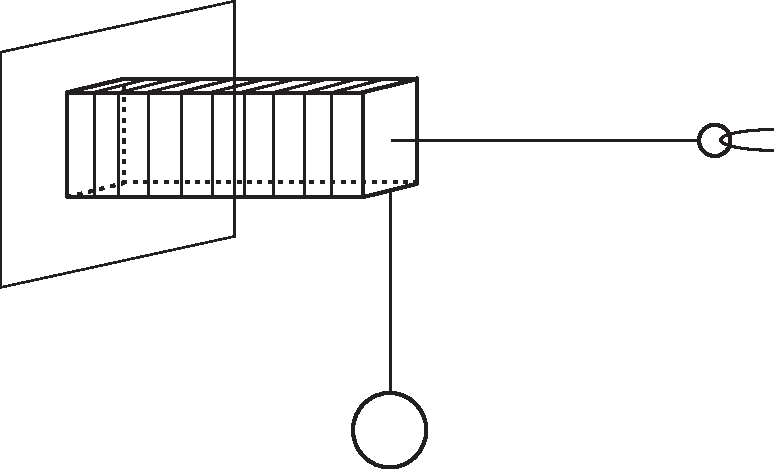
\includegraphics[width=0.5\textwidth]{images/LH037,04_051-052d-7.pdf}\\
\vspace*{0.5em}
\noindent \centering [\textit{Fig. 6}]
% \end{minipage}
% \hspace*{35mm}
\pend
\vspace*{1.5em}% PR: Rein provisorisch !!!
\pstart%
% \begin{minipage}[t]{0.2\textwidth}
% \hspace*{-5mm}
\centering%
\noindent%
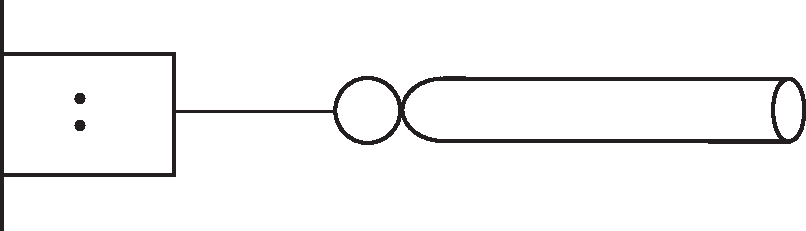
\includegraphics[width=0.5\textwidth]{images/LH037,04_051-052d-8.pdf}\\
%\vspace*{0.5em}
\noindent \centering [\textit{Fig. 7}]
% \end{minipage}
\pend
\count\Afootins=1500
\count\Bfootins=1500
\count\Cfootins=1500
%
%
%
%
% trabs
% resistentia respectiva
% divulsio
% centrum gravitatis
% ruptura 
% statera
% libra
% crassities
% murus
% tabula
% firmitas
% calculatio
% methodus
% ratiocinatio
% brachium